\documentclass{standalone}
\usepackage{tikz}
%\usetikzlibrary{...}
\begin{document}
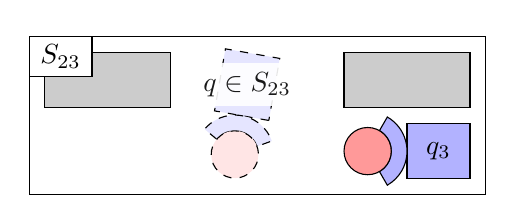
\begin{tikzpicture}

\draw (0,0) rectangle (5.8,2);

\draw[black,fill=black!20] (0.2,1.1) rectangle (1.8,1.8);
\draw[black,fill=black!20] (4.0,1.1) rectangle (5.6,1.8);

% robot (x1)
%\begin{scope}[shift={(0.6,0.55)}]
%   \draw[black,fill=blue!30] (0.0,-0.35) rectangle (0.8,0.35);
%   \node at (0.4,0) {$x_1$};
%   \draw[black,fill=blue!30,shift={(-0.5,0.0)}]
%      (-60:0.3) arc (-60:60:0.3) -- (60:0.5) arc (60:-60:0.5) -- cycle;
%   %\draw[black,fill=red!40] (-0.5,0) circle (0.3);
%\end{scope}

% robot (x2)
%\begin{scope}[shift={(4.8,0.55)},rotate=180]
%   %\draw[black,fill=blue!30] (0.0,-0.35) rectangle (0.8,0.35);
%   %\draw[black,fill=blue!30,shift={(-0.5,0.0)}]
%   %   (-60:0.3) arc (-60:60:0.3) -- (60:0.5) arc (60:-60:0.5) -- cycle;
%   \draw[black,fill=red!40] (-0.5,0) circle (0.3);
%\end{scope}

% robot (x3)
\begin{scope}[shift={(4.8,0.55)}]
   \draw[black,fill=blue!30] (0.0,-0.35) rectangle (0.8,0.35);
   \node at (0.4,0) {$q_3$};
   \draw[black,fill=blue!30,shift={(-0.5,0.0)}]
      (-60:0.3) arc (-60:60:0.3) -- (60:0.5) arc (60:-60:0.5) -- cycle;
   \draw[black,fill=red!40] (-0.5,0) circle (0.3);
\end{scope}

% robot (intermediate)
\begin{scope}[shift={(2.7,1.0)},rotate=80]
   \draw[black,fill=blue!10,dashed] (0.0,-0.35) rectangle (0.8,0.35);
   \draw[black,fill=blue!10,dashed,shift={(-0.5,0.0)}]
      (-60:0.3) arc (-60:60:0.3) -- (60:0.5) arc (60:-60:0.5) -- cycle;
   \draw[black,fill=red!10,dashed] (-0.5,0) circle (0.3);
   \node[fill=white,fill opacity=0.9] at (0.4,0) {$q \in S_{23}$};
\end{scope}

% label
\draw[fill=white] (0,1.5) rectangle (0.8,2);
\node at (0.4,1.75) {$S_{23}$};

% for vertical spacing
\node[inner sep=0] at (0,2.1) {};

\end{tikzpicture}%
\end{document}
